\documentclass[11pt,a4paper]{article}
\usepackage[top=3cm, bottom=2cm, left=2cm, right=2cm]{geometry}
\usepackage[utf8]{inputenc}
\usepackage{amsmath, amsfonts, amssymb}
\usepackage{siunitx}
\usepackage[brazil]{babel}
\usepackage{graphicx}
\usepackage[margin=10pt,font={small, it},labelfont=bf, textfont=it]{caption}
\usepackage[dvipsnames, svgnames]{xcolor}
\DeclareCaptionFont{MediumOrchid}{\color[svgnames]{MediumOrchid}}
\usepackage[pdftex]{hyperref}
\usepackage{natbib}
\bibliographystyle{plainnat}
\bibpunct{\textcolor{MediumOrchid}{\textbf{[}}}{\textcolor{MediumOrchid}{\textbf{]}}}{,}{s}{}{}
\usepackage{color}
\usepackage{footnote}
\usepackage{setspace}
\usepackage{booktabs}
\usepackage{multirow}
\usepackage{subfigure}
\usepackage{fancyhdr}
\usepackage{leading}
\usepackage{indentfirst}
\usepackage{wrapfig}
\usepackage{mdframed}
\usepackage{etoolbox}
\usepackage[version=4]{mhchem}
\usepackage{enumitem}
\usepackage{caption}
\usepackage{titlesec}
\usepackage{tcolorbox}
\usepackage{tikz}
\usepackage{LobsterTwo}
\usepackage[T1]{fontenc}
\usepackage{fontspec}
\usepackage{txfonts}
\usepackage[bottom]{footmisc}
\tcbuselibrary{skins,breakable}
\sisetup{output-decimal-marker={.}}

\makeatletter
\def\footnoterule{\kern-3pt\color{MediumOrchid}\hrule\@width0.6\textwidth height 0.8pt\kern2.6pt}
\makeatother

\renewcommand{\footnotelayout}{\itshape\color{MediumOrchid}}

\AtBeginEnvironment{equation}{\fontsize{13}{16}\selectfont}


\titleformat{\section}{\LobsterTwo\huge\color{CarnationPink}}{\thesection.}{1em}{}
\titleformat{\subsection}{\LobsterTwo\huge\color{CarnationPink}}{\thesubsection}{1em}{}
\titleformat{\subsubsection}{\bf\LobsterTwo\Large\color{MediumOrchid}}{\thesubsubsection}{1em}{}


\DeclareCaptionLabelFormat{figuras}{\textcolor{DarkTurquoise}{Figura \arabic{figure}}}
\captionsetup[figure]{labelformat=figuras}

\makeatletter
\renewcommand\tagform@[1]{\maketag@@@{\color{CarnationPink}(#1)}}
\makeatother

\renewcommand{\theequation}{Eq. \arabic{equation}}
\renewcommand{\thefigure}{Fig. \arabic{figure}}
\renewcommand{\thesection}{\textcolor{CarnationPink}{\arabic{section}}}

\setlist[itemize]{label=\textcolor{CarnationPink}{$\blacksquare$}}

\setlist[enumerate]{label=\textcolor{CarnationPink}{\arabic*.}, align=left, leftmargin=1.5cm}


\newcounter{exemplo}

\NewDocumentEnvironment{exemplo}{ O{} }{%
\allowbreak
\setlength{\parindent}{0pt}
  \begin{mdframed}[
  leftline=true,
  topline=false,
  rightline=false,
  bottomline=false,
  linewidth=2pt,
  linecolor=CarnationPink,
  frametitlerule=false,
  frametitlefont=\LobsterTwo\large\color{CarnationPink},
  frametitle={\color{CarnationPink}\LobsterTwo\large #1},
  ]
}{%
  \end{mdframed}
}

\setlength{\fboxsep}{5pt}
\setlength{\fboxrule}{1.5pt}
\usepackage{float}
\renewcommand{\thefootnote}{\alph{footnote}}
\usepackage{url}
\hypersetup{
	colorlinks=true,
	linkcolor=DarkTurquoise,
	filecolor=DarkTurquoise,      
	urlcolor=DarkTurquoise,
	citecolor=DarkTurquoise,
	pdftitle={Especialista em Física da Radioterapia}
}
\pagestyle{fancy}
\fancyhf{}
\renewcommand{\headrulewidth}{0pt}
\rfoot{\color{DarkTurquoise}\thepage \\ \LobsterTwo{\small\textcolor{CarnationPink}{@defDalila}}}

\title{\LobsterTwo\Huge{Braquiterapia}}
\author{\LobsterTwo\Large{Workflow em Braquiterapia}\nocite{*}}
\date{\LobsterTwo\textit{Dalila Mendonça}}
\begin{document}
	\maketitle

\section{Introdução}

	A braquiterapia é definida como a aplicação temporária ou permanente de pequenas fontes radioativas seladas próximas ou dentro do volume alvo. A distribuição da dose de tratamento é caracterizada por alta dose localizada e queda abrupta da dose. Logo depois que o rádio foi isolado quimicamente por Marie e Pierre Curie, os efeitos dos danos causados pela radiação na pele foram observados e levaram à primeira aplicação de material radioativo para o tratamento de tumores superficiais. 

	Algumas décadas depois, as agulhas de rádio foram usadas em implantes intersticiais de baixa dose. Os padrões de implante e os cálculos de dose foram realizados usando os sistemas de implantes Patterson-Parker ou Quimby. Embora esses métodos de cálculo de dose tenham sido retirados com a implementação de sistemas de planejamento de tratamento utilizando computadores, a geometria básica do implante desses sistemas ainda é usada.

	Atualmente, os sítos de tratamento predominantes para a braquiterapia são os cânceres de próstata, colo uterino, endométrio e irradiação parcial da mama. A Braquiterapia também é utilizada nos tratamentos intraoperatórios de irradiação parcial da mama e em algumas aplicações abdominais/pélvicas. Às vezes, a braquiterapia intersticial também é realizada para sarcomas de tecidos moles. 
	
	Com a implementação da radioterapia de intensidade modulada (IMRT), o uso de braquiterapia para tratamento de cânceres de cabeça e pescoço ou lesões brônquicas vem diminuindo. Da mesma forma, o acesso mais fácil à radioterapia com prótons diminuiu o uso da braquiterapia para melanomas oculares. 
	
	Os stents farmacológicos substituíram os tratamentos de braquiterapia intravascular (IVBT), embora mais recentemente a IVBT esteja sendo reconsiderada como terapia de resgate em casos de falhas dos stents medicamentosos. 
	
	Por outro lado, novos desenvolvimentos em aplicadores superficiais têm despertado um interesse no uso da braquiterapia para o tratamento de tumores superficiais. Vários grupos também estão trabalhando para desenvolver novos aplicadores para braquiterapia de câncer anal e retal. A \ref{fig:classificacoesBraqui} mostra o esquema de classificação para tratamentos de braquiterapia.

	\begin{figure}[h]
		\centering
		\fcolorbox{DarkTurquoise}{white}{%
			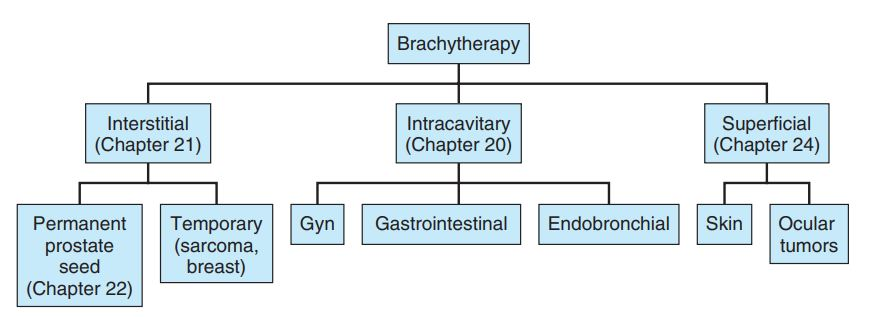
\includegraphics[width=0.6\textwidth]{Imagens/classificacoesBraqui.JPG}
		}%
		\caption{Esquema de classificação para tratamentos de braquiterapia.}
		\label{fig:classificacoesBraqui}
	\end{figure}

	
\section{Radioisótopos Utilizados em Braquiterapia}

	As primeiras fontes utilizadas para a braquiterapia foram o rádio e o radônio, que eram isótopos naturais. Com o advento dos isótopos produzidos artificialmente, muitas opções se tornaram disponíveis. Esses isótopos são produzidos através do bombardeamento de partículas em um reator nuclear (isótopos ricos em nêutrons) ou em um ciclotron (isótopos ricos em prótons) (\ref{fig:isotoposUtilizadosEmBraqu}).

	\begin{figure}[!ht]
		\centering
		\fcolorbox{DarkTurquoise}{white}{%
			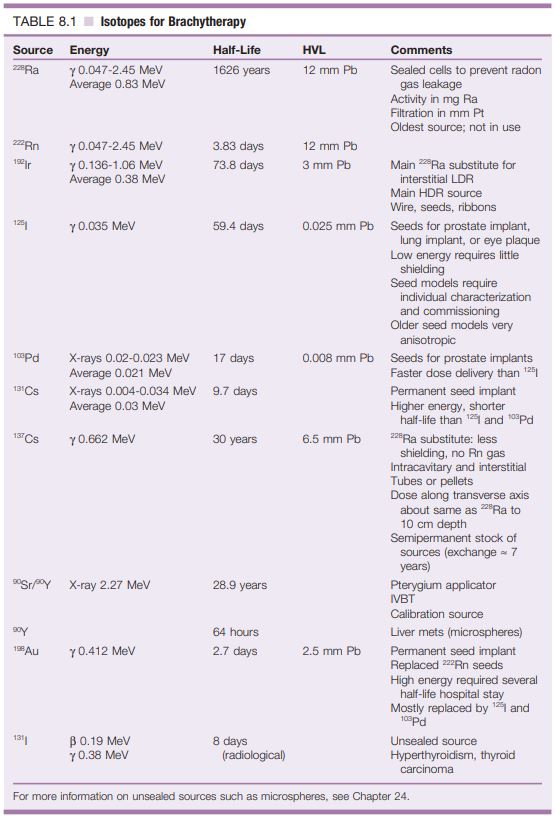
\includegraphics[width=0.7\textwidth]{Imagens/isotoposUtilizadosEmBraqu.JPG}
		}%
		\caption{Isótopos para Braquiterapia.}
		\label{fig:isotoposUtilizadosEmBraqu}
	\end{figure}
	

\section{Aplicadores em Braquiterapia}

	Existem muitos tipos de aplicadores de braquiterapia; um breve resumo é mostrado na \ref{fig:aplicadoresTipicos}.

	\begin{figure}[h]
		\centering
		\fcolorbox{DarkTurquoise}{white}{%
			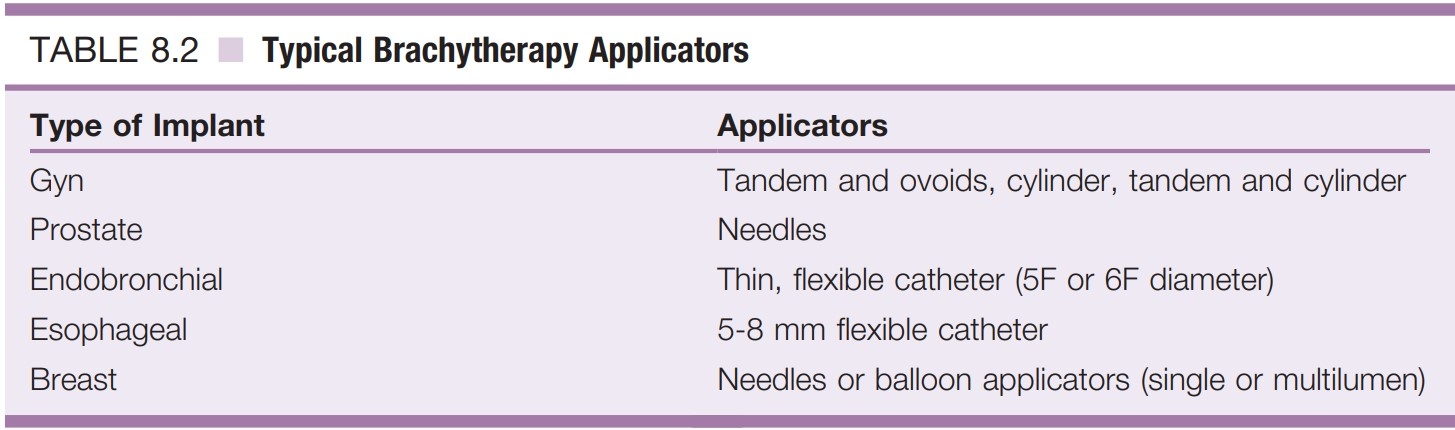
\includegraphics[width=0.8\textwidth]{Imagens/aplicadoresTipicos.jpg}
		}%
		\caption{Aplicadores típicos de braquiterapia.}
		\label{fig:aplicadoresTipicos}
	\end{figure}

\section{O Processo da Braquiterapia}

	A braquiterapia pode ser realizada de várias maneiras. Pode ser diferenciada pela taxa de dose, pelo tipo de implante e se o implante é temporário ou permanente. A baixa taxa de dose (LDR) é definida pela Comissão Internacional de Unidades e Medições de Radiação (ICRU)-38 como implantes que fornecem uma dose menor ou igual a 2 Gy/hora no ponto de prescrição. Da mesma forma o ICRU 38 define a braquiterapia de alta taxa de dose (HDR) como  implantes que fornecem uma dose maior ou igual a 12 Gy/hora no ponto de prescrição, embora a taxa de dose seja frequentemente muito maior. O tipo de implante pode ser intracavitário, intersticial ou superficial. E Finalmente, o implante pode ser permanente ou temporário. Os implantes permanentes apresentam inicialmente uma taxa de dose na faixa de 8 cGy/h até 32 cGy/hora, que decai exponencialmente de acordo com a meia-vida do radionuclídeo. A \ref{fig:aplicacoesDeBraquiterapia} mostra as aplicações típicas da braquiterapia.

	\begin{figure}[h]
		\centering
		\fcolorbox{DarkTurquoise}{white}{%
			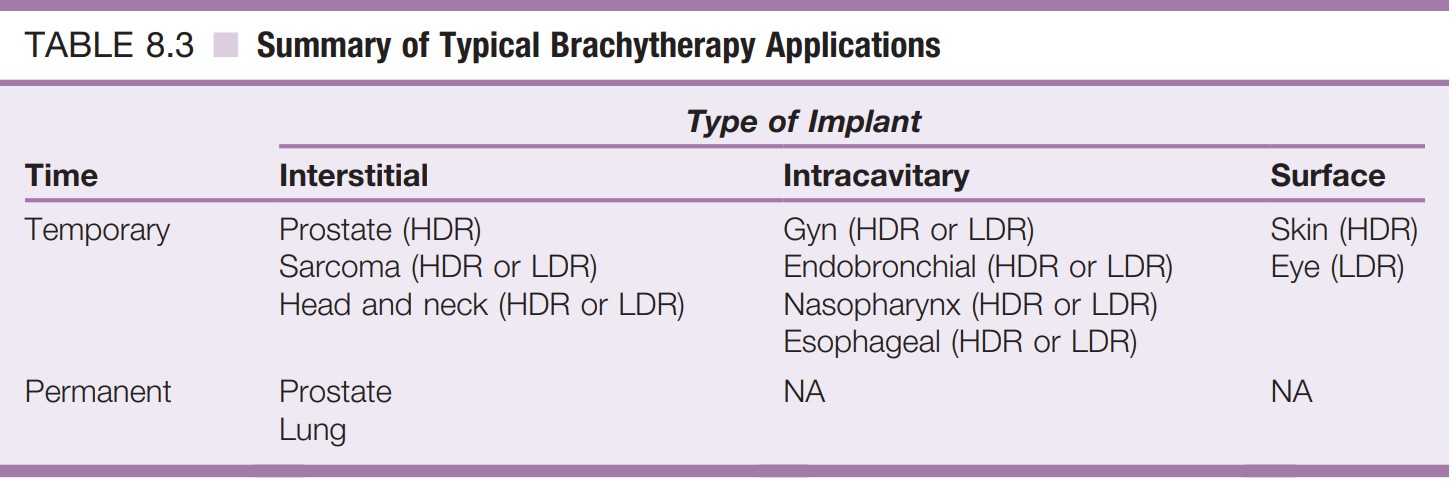
\includegraphics[width=0.8\textwidth]{Imagens/aplicacoesDeBraquiterapia.jpg}
		}%
		\caption{Principais aplicações de Braquiterapia.}
		\label{fig:aplicacoesDeBraquiterapia}
	\end{figure}

	A braquiterapia HDR é administrada usando afterloaders remotos. Esses sistemas possuem uma fonte de alta atividade fixa no final de um fio extenso. Quando a fonte não está em uso, ela é alojada em um invólucro altamente blindado. Normalmente, a fonte utilizada é de \ce{^{192}Ir}, com atividade típica variando de 10 Ci a 12 Ci no momento da instalação, embora fontes de \ce{^{60}Co} também estejam disponíveis. 
	
	
	Devido à meia-vida curta do 19\ce{^{192}Ir}2Ir, a fonte HDR é normalmente substituída a cada 3 meses. O aplicador é conectado à unidade HDR utilizando o que é chamado de tubo de transferência. Para implantes que utilizam múltiplos canais, algumas unidades de afterloading têm a capacidade de inserir o tubo de transferência em um canal específico, permitindo o tratamento apenas quando conectado ao canal correto. O fio da fonte é conduzido para fora do invólucro blindado e passa por vários aplicadores ou cateteres para entregar o tratamento. A posição onde a fonte para é chamada de posição de parada. A quantidade de tempo gasto em cada posição de parada é chamada de tempo de parada. Ambos os tratamentos, LDR e HDR, requerem salas blindadas.

	Os implantes temporários também podem ser realizados com fontes LDR (normalmente \ce{^{137}Cs}). Historicamente, este procedimento era feito carregando as fontes manualmente nos aplicadores ou cateteres, embora os afterloaders remotos LDR também estivessem disponíveis. 
	
	
	Os afterloaders movem o fio com a fonte para a posição de tratamento e, quando a equipe entra na sala de tratamento, o fio com a fonte se retrai. Depois que a equipe sai da sala, o tratamento é reiniciado. A LDR esteja é estudada principalmente para fins históricos, pois a maioria das instalações converteram seus tratamentos para HDR.

\section{Workflow Em Braquiterapia}

	Um fluxo de trabalho de braquiterapia genérico é mostrado na \ref{fig:workflowBraquiterapia}. As etapas são comuns para HDR e LDR, com exceção do pedido, recebimento e análise da fonte de LDR.
	
\subsection*{Planejamento Inicial e Prescrição do Tratamento}

	O planejamento inicial envolverá uma discussão sobre a seleção do aplicador e os objetivos do tratamento. A prescrição da dose será baseada no estágio do paciente e no tratamento combinado com radioterapia externa e/ou quimioterapia.

\subsection*{Pedido, Recebimento e Ensaios das Fontes}

	Para tratamentos LDR, deve haver um tempo para a aquisição de fontes. Para encomendar sementes nos Estados Unidos, o fornecedor deve ter uma cópia atualizada da licença de material radioativo da instalação que fica arquivada. Alguns radionuclídeos são produzidos apenas em quantidades limitadas uma vez por mês (por exemplo, sementes de \ce{^{125}I} em sutura para implantes pulmonares), portanto, pode ser necessário algum tempo de espera. Os fornecedores também podem ter um fornecimento limitado dos tipos mais raros de sementes (por exemplo, as sementes de \ce{^{125}I} de alta atividade utilizadas em placas oftalmológicas). 

	\begin{wrapfigure}{r}{0.36\textwidth}
		\centering
		\fcolorbox{DarkTurquoise}{white}{%
			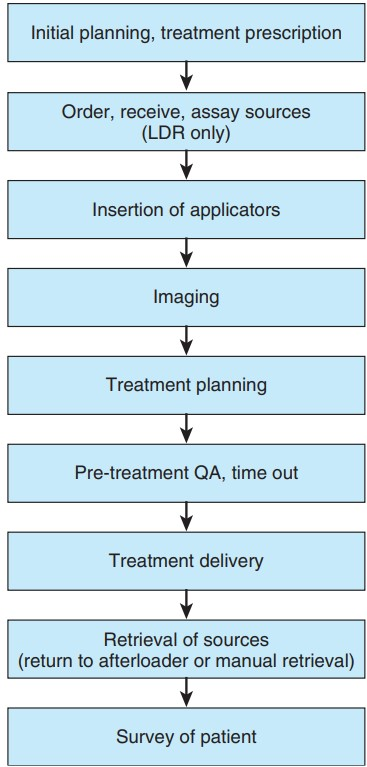
\includegraphics[width=0.25\textwidth]{Imagens/workflowBraquiterapia.jpg}
		}%
		\caption{Workflow}
		\label{fig:workflowBraquiterapia}
	\end{wrapfigure}

	Uma vez recebida, a embalagem deve ser inspecionada e verificada quanto a ausência de contaminação. Existem considerações especiais ao analisar fontes esterilizadas; a esterilidade deve ser mantida durante o ensaio ou então sementes extras do mesmo lote devem ser solicitadas para este fim.

\subsection*{Inserção de Aplicadores}

	
	A inserção do aplicador geralmente é um trabalho de equipe entre o cirurgião e o radio-oncologista, embora os implantes sejam cada vez mais realizados apenas pelo radio-oncologista. Para tratamentos LDR é fundamental ter um implante de qualidade porque não há possibilidade de otimização da distribuição de dose com base no posicionamento do implante. Já os tratamentos HDR podem aproveitar a posição de parada da fonte e a otimização do tempo de parada para compensar a geometria com qualidade abaixo do ideal, mas ainda é aconselhável usar uma boa técnica na inserção dos aplicadores, pois há limitações para a quantidade de otimização que pode ser realizada. Por exemplo, se a distância de uma determinada posição de parada até um órgão de risco for menor que a distância dessa posição de parada até o ponto de prescrição, a dose recebida no órgão de risco será sempre maior que a dose de prescrição. Outras posições de parada podem receber pesos maiores para neutralizar esse efeito, mas isso pode causar pontos quentes em outros locais.
	
	Ao realizar implantes planos ou volumétricos, é importante manter os cateteres a uma distância uniforme e paralelos entre si para minimizar pontos quentes ou pontos frios locais. Às vezes, os templates são utilizados para ajudar no espaçamento dos cateteres ou das agulhas. Por exemplo, os implantes de sementes para tratamentos de próstata utilizam templates. 

	Para massas em tecidos moles ou implantes mamários, uma agulha oca rígida pode ser utilizada para criar um caminho através do tecido e, em seguida, um cateter flexível com um travamento final pode ser inserido e a agulha removida.

\subsection*{Tipos de Imagens Utilizados em Braquiterapia}

	A principio, os planejamentos de braquiterapia era tradicionalmente feitos com radiografias 2D. Este tipo de imagem dificultava a determinação das posições dos cateteres, caso houvessem muitos, e não permitia a visualização das estruturas de tecidos moles, a menos que fosse utilizado um contraste para a aquisição das imagens. O contraste, às vezes, obscurecia os aplicadores e então eram adquiridas imagens antes e depois da administração de contraste. Além disso, para a braquiterapia ginecológica, recomenda-se a inserção de um cateter de Foley e a injeção de uma pequena quantidade de contraste no balão de Foley para auxiliar a identificação da bexiga.
	
	A reconstrução precisa das radiografias 2D requer um conhecimento preciso do centro do feixe, do fator de ampliação e da angulação do gerador de imagens para uma determinada fonte de raios-x. Gabaritos de reconstrução (jigs/ suportes) podem ser utilizados para auxiliar na reconstrução precisa das imagens ortogonais 2D. Esses suportes têm marcações de referência que definem a geometria e a amplificação das projeções, de modo que ao digitalizar esses pontos conhecidos no sistema, a geometria da fonte pode ser definida. O uso de TC e US tornaram-se o padrão para aquisição de imagens em braquiterapia e a ressonância magnética também está se tornando cada vez  mais comum.

	A espessura dos cortes da imagem é um ponto importante para ser possível delinear todo o comprimento do aplicador. Se a ponta do aplicador estiver totalmente dentro de um corte versus parcialmente dentro do corte, erros da ordem de metade da espessura do corte podem ser introduzidos. O espaçamento entre os cortes em uma TC de 2.5 mm a 3.0 mm é comumente utilizado. Para planos que utilizam vários canais, é importante identificar exclusivamente cada canal. Isso pode ser feito usando marcadores radiográficos fictícios (dummys) com um padrão único de marcadores curtos e longos. Para aplicadores como balões multilúmen utilizados em braquiterapia de mama, é importante garantir uma orientação consistente. Por exemplo, se o canal mais próximo da pele não for utilizado para minimizar a dose na pele, deve-se confirmar antes de cada tratamento que a orientação adequada se mantém.

\subsection*{Planejamento de Tratamento}

	O planejamento do tratamento para braquiterapia LDR envolve a determinação da taxa de dose. Com os aplicadores posicionados em uma geometria fixa, as únicas variáveis a serem otimizadas são a disponibilidade de fontes de \ce{^{137}Cs} com diferentes intensidades para os aplicadores ginecológicos e a disposição dessas fontes dentro dos aplicadores ou o número de sementes e sua posição dentro dos cateteres para implantes planares de \ce{^{192}Ir}, por exemplo. Para implantes volumétricos ou planares, a curva dose máxima com um contorno contíguo é utilizada para determinar a taxa de dose de tratamento. Esta é a curva de isodose mais alta que envolve o alvo sem se dividir. O tempo de tratamento é determinado simplesmente dividindo a dose total pela taxa de dose. Deve-se tomar cuidado para manter as taxas de dose em níveis aceitáveis, definidos historicamente sendo de 40cGy/h a 70 cGy/hora.

	O planejamento do tratamento para HDR aproveita a capacidade de otimizar a posição de parada da fonte e o seu o tempo de parada em qualquer lugar ao longo do comprimento do aplicador. O artigo de Thomadsen\cite{thomadsen2008anniversary} tem uma discussão sobre as técnicas de otimização. O artigo lista alguns princípios gerais para otimizar os implantes intersticiais, o que não é exclusivo da braquiterapia HDR, mas é mais aplicável a HDR devido a sua flexibilidade na otimização. 
	
	Os princípios da braquiterapia intersticial são:

	\begin{itemize}[label=\textcolor{CarnationPink}{$\blacktriangleright$}]
		\item Para alcançar distribuições de dose mais uniformes, a concentração das fontes ou as posições de parada precisam ser maiores perto das periferias (isto é, carregamento periférico). Até 75\% da atividade pode estar nas posições periféricas, mas isto dependerá da forma do volume alvo clínico (CTV) e das posições da fonte.
		\item As agulhas nos cantos dos implantes devem ser movidas para dentro para evitar quebras nas linhas de isodose. Reduzir a distância para cerca de dois terços da distância utilizadas no padrão geométrico regular geralmente é suficiente.
		\item Ao usar sementes pequenas, a força das fontes localizadas nas extremidades das agulhas precisa ser o dobro das outras localizações da agulha. Para implantes de semente de próstata, isso é obtido colocando as fontes uma atrás da outra nas extremidades distal e proximal da agulha.
	\end{itemize}

	Os princípios da braquiterapia intracavitária são:

	\begin{itemize}[label=\textcolor{CarnationPink}{$\blacktriangleright$}]
		\item Quando o objetivo é projetar a dose para pontos distantes do aplicador, as posições das fontes devem estar distantes da interface aplicador-tecido. Isso se deve ao efeito do inverso quadrado da distância. Assim como uma maior distância fonte-superfície (SSD) na teleterapia produz uma dose na profundidade mais alta, uma distância fonte-tecido maior na braquiterapia também produz uma dose maior na profundidade. Por exemplo, a escolha de um cilindro com um diâmetro maior resultará em doses mais altas à distância em relação à dose na superfície do cilindro.
		\item Se possível, o arranjo do aplicador deve colocar as fontes ao redor do alvo (ou seja, usar tandem e ovoides versus tandem e cilindro).
		\item A distribuição da dose não será uniforme, mas diminuirá continuamente com a distância até as fontes.
	\end{itemize}

	Para o planejamento HDR utilizando aplicadores (por exemplo, cilindros), a distância de prescrição deve ser maior que o espaçamento das posições das fontes para limitar a ondulação nas linhas de isodose.

\subsection*{QA Pré-Tratamento e Time-Out}

	O AAPM TG-59, \textbf{\textit{``High Dose-Rate Brachytherapy Treatment Delivery''}}, descreve o QA pré-tratamento para um procedimento de braquiterapia HDR. Embora essas etapas sejam específicas para HDR, os princípios gerais também se aplicam à braquiterapia LDR.

	\begin{enumerate}[label=\textcolor{CarnationPink}{\roman*.}]
		\item Duas pessoas devem verificar a conexão adequada dos cateteres à unidade HDR e verificar se os tubos de transferência estão livres de dobras.
		\item O kit de emergência e o container da fonte devem estar disponíveis.
		\item Verificar se o monitor de área está presente e de forma operacional. (Não mencionado no AAPM TG-59, mas a recomendação é examinar o paciente antes do tratamento para confirmar o background. O paciente pode ter feito uma aquisição de medicina nuclear antes do tratamento, causando uma leitura elevada. Se isto não for avaliado antes do tratamento, pode acarretar em uma confusão ao realizar o monitoramento pós-tratamento).
		\item Verificar se os comprimentos dos tubos de transferência estão corretos.
		\item Verificar o posicionamento do aplicador. Isso pode ser feito pela verificação das medidas realizadas no momento da inserção (ou seja, distância do template à extremidade proximal da agulha) ou posicionamento do tandem comparado com as marcas na pele do paciente.
		\item Revisão da documentação do tratamento:
			\begin{enumerate}[label=\textcolor{CarnationPink}{(\alph*)}]
				\item Verificar se o plano e prescrição estão assinados.
				\item Certificar se a segunda verificação foi realizada.
				\item Verificar se o plano está de acordo com a prescrição.
				\item Caso seja aplicável, verificar se o plano atual condiz com as frações anteriores.
				\item Verificar se as posições e os tempos de parada do plano estão de acordo com o que está programado no console de tratamento. Nos casos de LDR, verificar se foi realizado o duplo check do carregamento da fonte.
			\end{enumerate}
		\item Identificação do paciente por dois parâmetros diferentes (normalmente o nome e a data de nascimento).
	\end{enumerate}

	Além disso, é uma boa prática fazer um pequeno intervalo antes de iniciar o tratamento para garantir que toda a equipe que participa do tratamento estão de acordo que os parâmetros a serem entregues estão corretos, que a paciente correta está sendo tratada no local correto, que a equipe estejam com seus monitores individuais de exposição e que os dispositivos de resposta à emergências foram identificados.

\subsection*{Entrega do Tratamento}

	Os \textcolor{MediumOrchid}{\textbf{tratamentos LDR}} podem ser entregues através afterloader remoto porém o carregamento manual é a forma mais comum de carregamento. Como o carregamento é feito manualmente, ele deve ser bem pensado para que o tempo de inserção seja minimizado e consequentemente a exposição da equipe também seja minimizada. 

	O carregamento da fonte deve ser verificado por duas pessoas. Isso inclui dispor antecipadamente as ferramentas apropriadas com um acesso mais fácil, removendo as capas dos aplicadores e garantindo que não exista nenhuma obstrução no espaço de trabalho. 
	
	As entregas de braquiterapia LDR podem durar de 1 dia até 3 dias. Isso requer que o paciente seja internado em uma sala blindada. Blindagens portáteis podem ser utilizadas para aumentar a blindagem da sala. 
	
	A equipe deve ser instruída quanto à prática de segurança ao cuidar desses pacientes. Uma forma é limitando a quantidade de tempo que a equipe assistencial permanece à beira do leito, pois a menos que esteja sendo prestado cuidado direto ao paciente, não há necessidade de estar por longos períodos ao lado do leito; Outra forma que diminui significativamente a exposição da equipe é instruindo a equipe a se afastar do paciente ao se comunicar (dano vários passos para trás, por exemplo). As unidades de afterloading remoto eliminam esse problema, pois as fontes são removidas quando a equipe entra na sala. Um levantamento radiométrico das áreas circunvizinhas deve ser feito para confirmar que todos os níveis de radiação são aceitáveis.

	Os \textcolor{MediumOrchid}{\textbf{tratamentos HDR}} normalmente levam de 5 a 15 minutos, dependendo da intensidade da fonte e do tipo de tratamento, embora os tratamentos interoperatórios possam ser muito mais longos. De acordo com os regulamentos da NRC, um físico médico autorizado e um usuário autorizado (radio-oncologista) devem estar presentes durante o tratamento. A equipe deve ser treinada para o caso de ocorrer uma emergência em que a fonte fique presa dentro de um aplicador, de modo que eles consigam responder a esta situação:

	\begin{enumerate}[label=\textcolor{CarnationPink}{\arabic*${}^\circ$}]
		\item O primeiro passo da ação é pressionar a o botão de emergência na tentativa de forçar a retração da fonte;
		\item Caso o \textcolor{CarnationPink}{$\mathrm{1^{\circ}}$} não funcionar, o membro treinado da equipe deve entrar na sala e tentar retornar a fonte para a posição protegida usando o método de retração manual (manivela).
		\item Caso o \textcolor{CarnationPink}{$\mathrm{2^{\circ}}$} não funcionar, o médico deverá entrar na sala e remover o aplicador com a fonte ainda nele e colocar a fonte no envólucro de emergência.
		\item O paciente deve ser removido da sala e ser examinado imediatamente para confirmar que a fonte foi de fato removida do paciente.
		\item A sala deve ser protegida (marcada com “não entre”) e o fornecedor deve ser notificado.
		\item A exposição não intencional da equipe deve ser estimada. As leituras reais podem ser obtidas quando os monitores individuais de exposição da equipe são lidos.
	\end{enumerate}

	O AAPM TG-59 fornece uma estimativa das exposições devido a uma fonte de 10 Ci para vários tempos e distâncias. Por exemplo, em 10 minutos um indivíduo receberia 750 mGy a 10 cm da fonte, 30 mGy a 50 cm e 7.5 mGy a 100 cm. Comparando esses valores com o limite anual permitido de 50 mSv (mSv = mGy para fótons), pode-se observar que uma resposta de emergência eficiente não resultará em uma exposição excessiva da equipe, porém pode resultar em uma dose não intencional significativa no paciente.

	Para minimizar a chance de ocorrer uma emergência devido à uma fonte presa, todas as unidades HDR têm um fio com uma dummy (fonte fictícia) que é enviada antes da fonte radioativa para confirmar que o caminho não está obstruído. Caso for encontrada alguma resistência durante a simulação de tratamento com a dummy, um alarme é ativado.
	
	Pode haver opções sobre como as execuções com a dummy são configuradas. Para um implante de múltiplos canais, é desejável confirmar que todos os canais estão livres de obstrução antes de tratar qualquer canal. Isso impede que um tratamento parcial seja entregue caso um dos canais tenham uma obstrução. Algumas unidades oferecem uma configuração de dupla verificação que primeiramente verifica todos os canais antes de iniciar o tratamento do primeiro canal e verifica individualmente cada canal imediatamente antes de ser utilizado com a fonte radioativa. Deve-se tomar o cuidado de manter os tubos de transferência o mais retos possível para minimizar a chance de torcer um tubo e causar uma obstrução.

\subsection*{Recuperação de Fontes, Monitoramento Pós-Tratamento e Revisão de Registros}

	Para tratamentos LDR com carregamento manual, as fontes são simplesmente removidas dos aplicadores. Assim como o carregamento, o processo de remoção das fontes deve ser bem pensado e eficiente. O invólucro de armazenamento deve ser colocado próximo a uma área de trabalho desobstruída e após a remoção da fonte, os aplicadores são removidos. Para tratamentos HDR, a fonte retorna à posição protegida após a conclusão do tratamento e na sequência, os tubos de transferência podem ser desconectados e os aplicadores removidos.

	Um monitoramento pós-tratamento do paciente e da área onde ocorreu o tratamento é exigido pelo NRC (10 CFR 35.604 para afterloaders remotos e 10 CFR 35.404 para carregamento manual) para confirmar que nenhuma fonte permanece dentro do paciente e que as fontes não foram inadvertidamente descartadas. Uma revisão de todos os registros deve ser feita para garantir que tudo esteja completo. Para tratamentos de afterloading remoto, o registro de pós-tratamento deve ser revisado para confirmar se o que foi entregue corresponde ao que foi planejado.

\section{QA do Processo de Braquiterapia}

	O AAPM TG-56, \textit{\textbf{``Code of Practice for Brachytherapy''}}, recomenda o desenvolvimento de um programa de controle de qualidade para todo o processo de braquiterapia. Os objetivos buscados em um programa de QA são:

	\begin{enumerate}
		\item Garantir que cada tratamento individual seja administrado de forma consistente;
		\item Garantir que cada tratamento reflita com precisão a intenção clínica do radio-oncologista; e
		\item Garantir que cada tratamento seja executado com respeito à segurança do paciente e da equipe.
	\end{enumerate}

	O programa de QA deve abordar três processos básicos: \textcolor{MediumOrchid}{$\mathbf{(i)}$} inserção do aplicador, \textcolor{MediumOrchid}{$\mathbf{(ii)}$} design e avaliação do implante e \textcolor{MediumOrchid}{$\mathbf{(iii)}$} o processo de entrega do tratamento. O TG-56 descreve quatro categorias para os end-points do programa de QA:

	\begin{enumerate}[label=\textcolor{CarnationPink}{(\roman*)}]
		\item \textcolor{DarkTurquoise}{\textbf{Segurança do paciente, do público e da instituição.}} Isso inclui o controle da exposição, o fornecimento de proteção adequada e os procedimentos para manter sob controle todas as fontes radioativas. Os usuários devem ter a capacidade de reconhecer uma situação de perigo e também devem saber como responder em casos de emergência. Para afterloaders remotos, o controle de qualidade envolverá a verificação da operação de todos os intertravamentos. A conformidade regulatória, embora necessária, não necessariamente aborda a segurança.
		
		\item \textcolor{DarkTurquoise}{\textbf{Precisão espacial (posicionamento da fonte).}} A posição da fonte ou posição de parada ativa, conforme definida pelo médico, deve ser verificada. Esta verificação normalmente é feita em relação à marcadores dummy e, portanto, a equipe deve entender como cada sistema determina as posições de parada. Por exemplo, um sistema Varian, pode precisar que o ponto mais distal do cateter seja identificado, enquanto um sistema da Elekta, pode precisar que o centro da posição mais distal da fonte seja marcado. A NRC estabelece uma precisão de $\pm$ 1 mm para os testes de posição da fonte, porém isso pode não ser possível na prática clínica devido à incertezas na localização do cateter.
		
		\item \textcolor{DarkTurquoise}{\textbf{Precisão temporal.}} Nesse caso, um limite de $\pm$2 \% para medidas temporais é facilmente alcançável. A dose em trânsito deve ser avaliada e, se necessário, devem ser feitas correções temporais para compensar a dose entregue em transito (dose entregue na movimentação da fonte não contabilizada na dose entregue).
		
		\item \textcolor{DarkTurquoise}{\textbf{Precisão na entrega da dose.}} O requisito principal é uma calibração precisa da atividade da fonte. Além disso devem ser uitilizados os parâmetros adequados para os cálculo da fonte. A atenuação do aplicador e o efeito das blindagens devem ser considerados, se possível. A precisão da reconstrução 3D dos aplicadores deve ser confirmada. A precisão dos pontos de referência de dose (ou seja, Ponto A) e a precisão pontos de referência dos órgãos de risco (ou seja, reto e bexiga) também terão impacto na qualidade do plano.
	\end{enumerate}

	O AAPM TG-56 também enfatiza que cada instituição precisará desenvolver seu próprio processo de controle de qualidade, mas que esses fatores acima devem ser abordados. Para o controle de qualidade específico do procedimento, regras e guidelines devem ser desenvolvidos para definir a ordem cronológica do processo e limitar a gama de possíveis ações para cada etapa para minimizar a chance de erros. Verificações redundantes e um fluxo de trabalho cuidadosamente projetado também devem ser desenvolvidos. 
	
	O TG-56 descreve também um processo passo a passo para desenvolver QA procedimento-específico:

	\begin{enumerate}[label=\textcolor{CarnationPink}{\arabic*${}^\circ$}]
		\item Definir o fluxo de trabalho. Em cada etapa, deve-se identificar os membros da equipe envolvidos, as atividades críticas e as informações a serem registradas.
		\item Utilização de uma documentação cuidadosamente elaborada para garantir uma comunicação precisa e formar a base para o registro permanente do tratamento.
		\item Identificar os pontos vulneráveis no processo de entrega do tratamento e criar verificações redundantes.
		\item Desenvolver um procedimento escrito que descreva a ordem cronológica do procedimento, as funções dos membros da equipe, as verificações de controle de qualidade e a documentação associada. É recomendado os check-lists de verificação.
		\item Integração ao programa geral de controle de qualidade. Instituir uma auditoria independente aleatória de amostras de registros de pacientes e uma revisão de quaisquer erros. Desenvolver um processo formal de melhoria da qualidade clínica (CQI).
	\end{enumerate}

\section{Cálculos de Dose}

	
	O método de cálculo de dose mais aceito atualmente é o descrito pelo AAPM TG-43. A equação geral para a taxa de dose 2D é:

	$$\dot{D} (r, \theta) = S_{k} \cdot \Lambda \cdot \left(\frac{G_{L}(r, \theta)}{G_{L}(r_0, \theta_0)}\right) \cdot g_{L}(r) \cdot F(r, \theta) $$

	\begin{exemplo}[onde:]
		\begin{itemize}[label=\textcolor{CarnationPink}{$\star$}]
			\item \textcolor{DarkTurquoise}{$\mathbf{S_{k}}$:} Força kerma no ar em unidade de U (onde U $=$ \unit{\mu Gy \; m^2 \; h^{-1}} $=$ \unit{c Gy \; cm^2 \; h^{-1}});
			\item \textcolor{DarkTurquoise}{$\mathbf{\Lambda}$:} Constante de taxa de dose na água dada em \unit{cGy \; h^{-1} U^{-1}};
			\item \textcolor{DarkTurquoise}{$\mathbf{r}$:} Distância em cm;
			\item \textcolor{DarkTurquoise}{$\mathbf{r_0}$:} Distância de referência igual a 1 cm;
			\item \textcolor{DarkTurquoise}{$\mathbf{\theta}$:} Ângulo polar em relação ao eixo longitudinal da fonte linear;
			\item \textcolor{DarkTurquoise}{$\mathbf{G_{L}(r, \theta)}$:} Função geométrica (modelo aproximado para a efetiva lei do inverso quadrado);
			\item \textcolor{DarkTurquoise}{$\mathbf{G_{L}(r_0, \theta_0)}$:} Função geométrica na distância e no ângulo de referência (\ang{90})
			\item \textcolor{DarkTurquoise}{$\mathbf{ g_{L}(r)}$:} Função de dose radial (queda de dose devido ao espalhamento e atenuação);
			\item \textcolor{DarkTurquoise}{$\mathbf{ F(r, \theta)}$:} Função de anisotropia (variação na dose em função do ângulo polar para levar em conta o encapsulamento e a forma da fonte, é igual a 1 para $\mathrm{\theta_0}$).
		\end{itemize}
	\end{exemplo}

	Todos os parâmetros são específicos para o modelo da fonte e deve-se tomar cuidado para garantir que os valores corretos sejam utilizados nos cálculos. Os valores de consenso estão disponíveis no site do IROC-Houston (anteriormente RPC).
	
	Para uma fonte pontual, a equação se torna:

	$$\dot{D} (r) = S_{k} \cdot \Lambda \cdot \left(\frac{G_{L}(r, \theta_0)}{G_{L}(r_0, \theta_0)}\right) \cdot g_{L}(r) \cdot \phi_{an}(r)$$

	\begin{exemplo}[onde:]
		\begin{itemize}[label=\textcolor{CarnationPink}{$\star$}]
			\item \textcolor{DarkTurquoise}{$\mathbf{\phi_{an}(r)}$:} Função de anisotropia 1D dada como a taxa de dose média ponderada pelo ângulo sólido ao longo de todo o ângulo sólido de $\mathrm{4\pi}$. O relatório original da AAPM TG-43 exigia uma constante de isotropia independente de r, mas não é mais recomendado.
		\end{itemize}		
	\end{exemplo}

	A função geométrica é dada por:

	$$G(r, \theta) = \begin{cases}
		\frac{\beta}{L \; r \sin(\theta)}, & \text{ se } \theta \neq 0 \\

		\\

		\left(\frac{r^2 - L^2}{4}\right)^{-1}, & \text{ se } \theta = 0 \\

		\\

		r^{-2}, & \text{ se } \text{fonte pontual}
	\end{cases}$$

	\begin{exemplo}[onde:]
		\begin{itemize}[label=\textcolor{CarnationPink}{$\star$}]
			\item \textcolor{CarnationPink}{$\mathbf{\beta}$} é o ângulo em radianos subtendido pelas extremidades da fonte linear em relação ao ponto de cálculo; e
			\item \textcolor{CarnationPink}{$\mathbf{L}$} é o comprimento ativo da fonte.
		\end{itemize}		
	\end{exemplo}

	A função de dose radial é tabelada com base na distância do ponto até a fonte e caso necessário deve ser feita uma interpolação para derivar o valor necessário. A função de anisotropia é tabelada com base na distância e do ângulo formado com a fonte. 

	À distâncias próximas a uma fonte linear, a queda de dose é menor do que seria esperado através da lei do inverso quadrado da distância devido ao fato de que os fótons que emergem das extremidades da fonte percorrem uma distância maior e atravessam por mais filtração em uma incidência oblíqua. Como regra geral, em distâncias $>$ que 2 vezes o comprimento da fonte, a distribuição de dose da fonte linear seguirá a lei do inverso quadrado da distância.

	Como já mencionado, todos esses valores são dependentes do modelo da fonte e as fórmulas para cálculos da fonte linear e fonte pontual são modelos aproximados para a distribuição uniforme da atividade em uma fonte. Estes parâmetros não incluem efeitos como a absorção diferencial no encapsulamento. Além disso, os cálculos de dose com base no formalismo modular do TG-43 não permite atenuação fonte-a-fonte e nem faz correções para a heterogeneidade do tecido. 

\section{Especificação e Report da Dose}

	A \ref{fig:especificacaoDeDoseImplante} mostra os pontos típicos para a especificação da dose para vários tipos de implantes. O uso do planejamento 3D substitui as especificações simples de dose pontual por especificações volumétricas semelhantes à teleterapia.

	\begin{figure}[h]
		\centering
		\fcolorbox{DarkTurquoise}{white}{%
			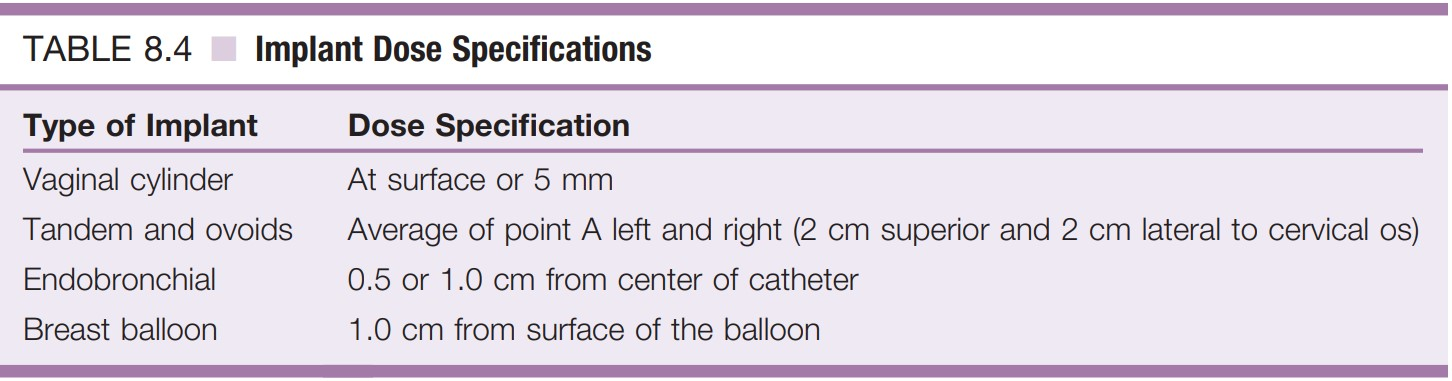
\includegraphics[width=0.8\textwidth]{Imagens/especificacaoDeDoseImplante.jpg}
		}%
		\caption{Especificações de dose para diferentes implantes.}
		\label{fig:especificacaoDeDoseImplante}
	\end{figure}

	Para braquiterapia intracavitária, o ICRU-38 recomenda reportar as seguintes quantidades:

	\begin{enumerate}[label=\textcolor{CarnationPink}{(\roman*)}]
		\item As dimensões do contorno da isodose de 60 Gy, incluindo a dose entregue pelo feixe externo;
		\item A dose em um ponto da bexiga localizado na superfície posterior do balão de Foley na linha média anterior/posterior definida no centro do balão;
		\item A dose em um ponto retal localizado a 0.5 cm posterior à cavidade vaginal em uma linha anterior/posterior na metade da distância entre as fontes vaginais;
		\item Doses nos pontos que representam os gânglios linfáticos para-aórticos, comuns e ilíacas externas;
		\item Doses nos pontos que representam o paramétrio distal e os linfonodos obturadores.
	\end{enumerate}

	Conforme apontado no AAPM TG-56, o volume do contorno da isodose de 60 Gy não mostrou correlação com as dimensões das fontes individuais, mas sim com a atividade total implantada. O AAPM TG-56 recomenda que o kerma no ar integrado de referência (IRAK - \textit{``integrated reference air kerma''}) seja reportado. O IRAK é a força kerma-ar total do implante multiplicada pelo tempo de tratamento para cada fonte utilizada. O tempo deve estar em segundos para tratamentos HDR e em horas para tratamentos LDR. O processo de especificação da dose em uma instalação deve ser bem descrito e compreendido por todos os funcionários envolvidos no processo de planejamento. As convenções para localização dos pontos de referência devem ser bem documentadas. Variações nas formas de especificação da dose e nas práticas de planejamento de tratamento não são recomendada. Esses fatores são desenvolvidos para funcionar como um sistema e os resultados não podem ser previstos se o sistema não for utilizado em sua totalidade.

	O ICRU-58 especifica os guidelines para a braquiterapia intersticial conforme apresentado na \ref{fig:recomendacaoIcruReportIntersticial}. Além disso, o ABS recomenda relatar a metodologia de planejamento (ou seja, Manchester, Paris, nomograma do Memorial, modelo personalizado, otimização, etc.).

	\begin{figure}[h]
		\centering
		\fcolorbox{DarkTurquoise}{white}{%
			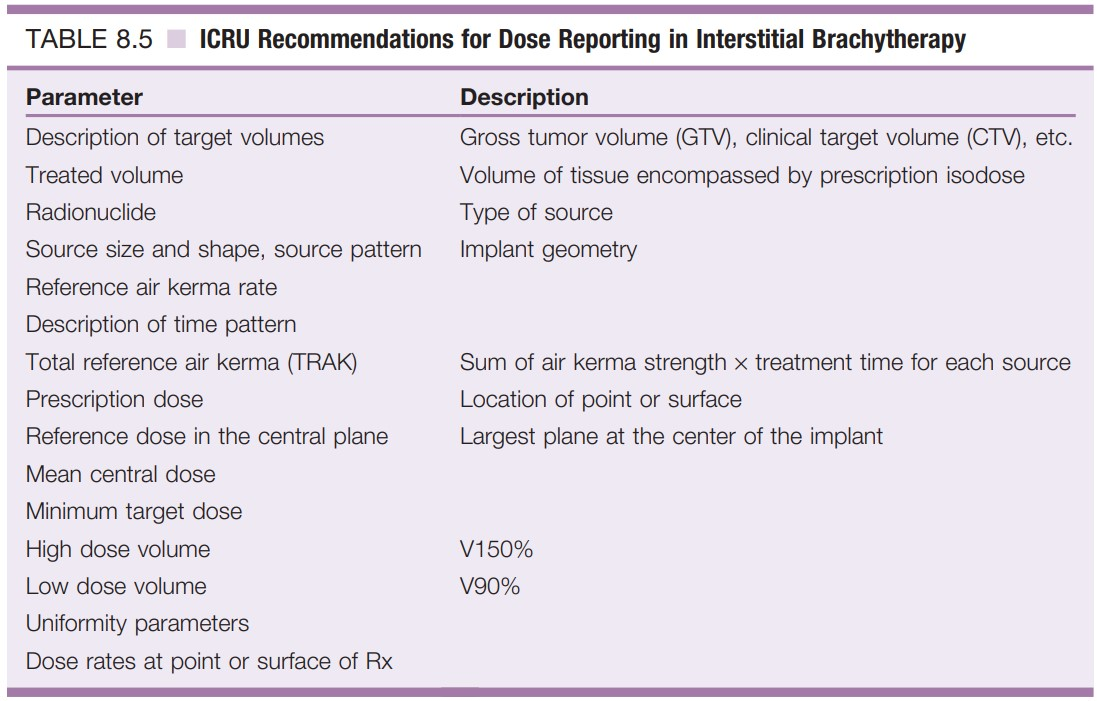
\includegraphics[width=0.8\textwidth]{Imagens/recomendacaoIcruReportIntersticial.jpg}
		}%
		\caption{Recomendações do ICRU-58 para o report de doses em braquiterapia intersticial.}
		\label{fig:recomendacaoIcruReportIntersticial}
	\end{figure}


\section{Manuseio, Transporte, Armazenamento e Inventário das Fontes}

	A taxa de dose na superfície de uma fonte radioativa pode ser extremamente alta e, portanto, as fontes nunca devem ser diretamente manuseadas. Fórceps ou pinças de cabo longo devem ser utilizados para o manuseio das fontes. As fontes devem ser enviadas de acordo com os regulamentos da CNEN. Para poder transportar materiais radioativos para fora da instalação, é necessária uma licença. 

	Materiais radioativos devem estar sob o controle da instalação em todos os momentos. Isso significa que deve estar ou sob controle direto ou seguro em uma área trancada. Além disso, a instalação deve ter um rigoroso controle de estoque e deve documentar a localização de todos os materiais radioativos em todos os momentos. Quando as remessas são recebidas, as fontes devem ser registradas em um inventário.
	
	Caso as fontes forem removidas da área de armazenamento para serem levadas para a área de tratamento, o registro deve conter quais fontes foram coletadas, qual o destino das fontes, a data e a hora da coleta e quem as coletou. Se nem todas as fontes forem utilizadas para o tratamento, todas as fontes devolvidas à área de armazenamento devem ser registradas novamente. Da mesma forma, após a conclusão do tratamento, todas as fontes devem ser devolvidas à área de armazenamento e novamente registradas no inventário.
	
	Os radionuclídeos de vida curta podem ser devolvidos ao fornecedor para posterior descarte ou podem permanecer armazenados na área de armazenamento até decairem 10 meias-vidas antes de ser feito seu descarte como lixo normal. Caso uma fonte seja enviada de volta ao fornecedor, a instalação deverá receber e manter armazenada a confirmação de recebimento da fonte pelo fornecedor.
	
\bibliography{ref.bib}
\end{document}